% This section describes the design of the memory system model. How host target
% decoupling is achieved. What configurations are available.

Our memory system model \textit{generator} describes a space of individual
\textit{instances} that model different memory systems. Implemented in
Chisel\cite{Chisel}, the generator emits a host-decoupled module that is
attached to other simulation models during simulation mapping. All instances
are runtime-configurable via memory-mapped registers that presented on the
MIDAS simulation interconnect.

Instances operate by using the FPGA host's off-chip memory system as a backing
store: target requests carried through simulation tokens are snooped by the
\emph{ingress unit} and re-issued to the host memory system. Reponses from the
host memory system are subsequently saved by the \emph{egress unit}.  In
parallel, a host-decoupled \emph{timing model} explicitly consumes input tokens
and generates output tokens. When the timing model wishes to release a token
with a valid target response, it fetches the matching host response from the
egress unit. If no host response is present, the timing model does not produce
a token, thus, simulation timing is maintained regardless of host-memory system
timing.

\begin{figure}
	\centering
	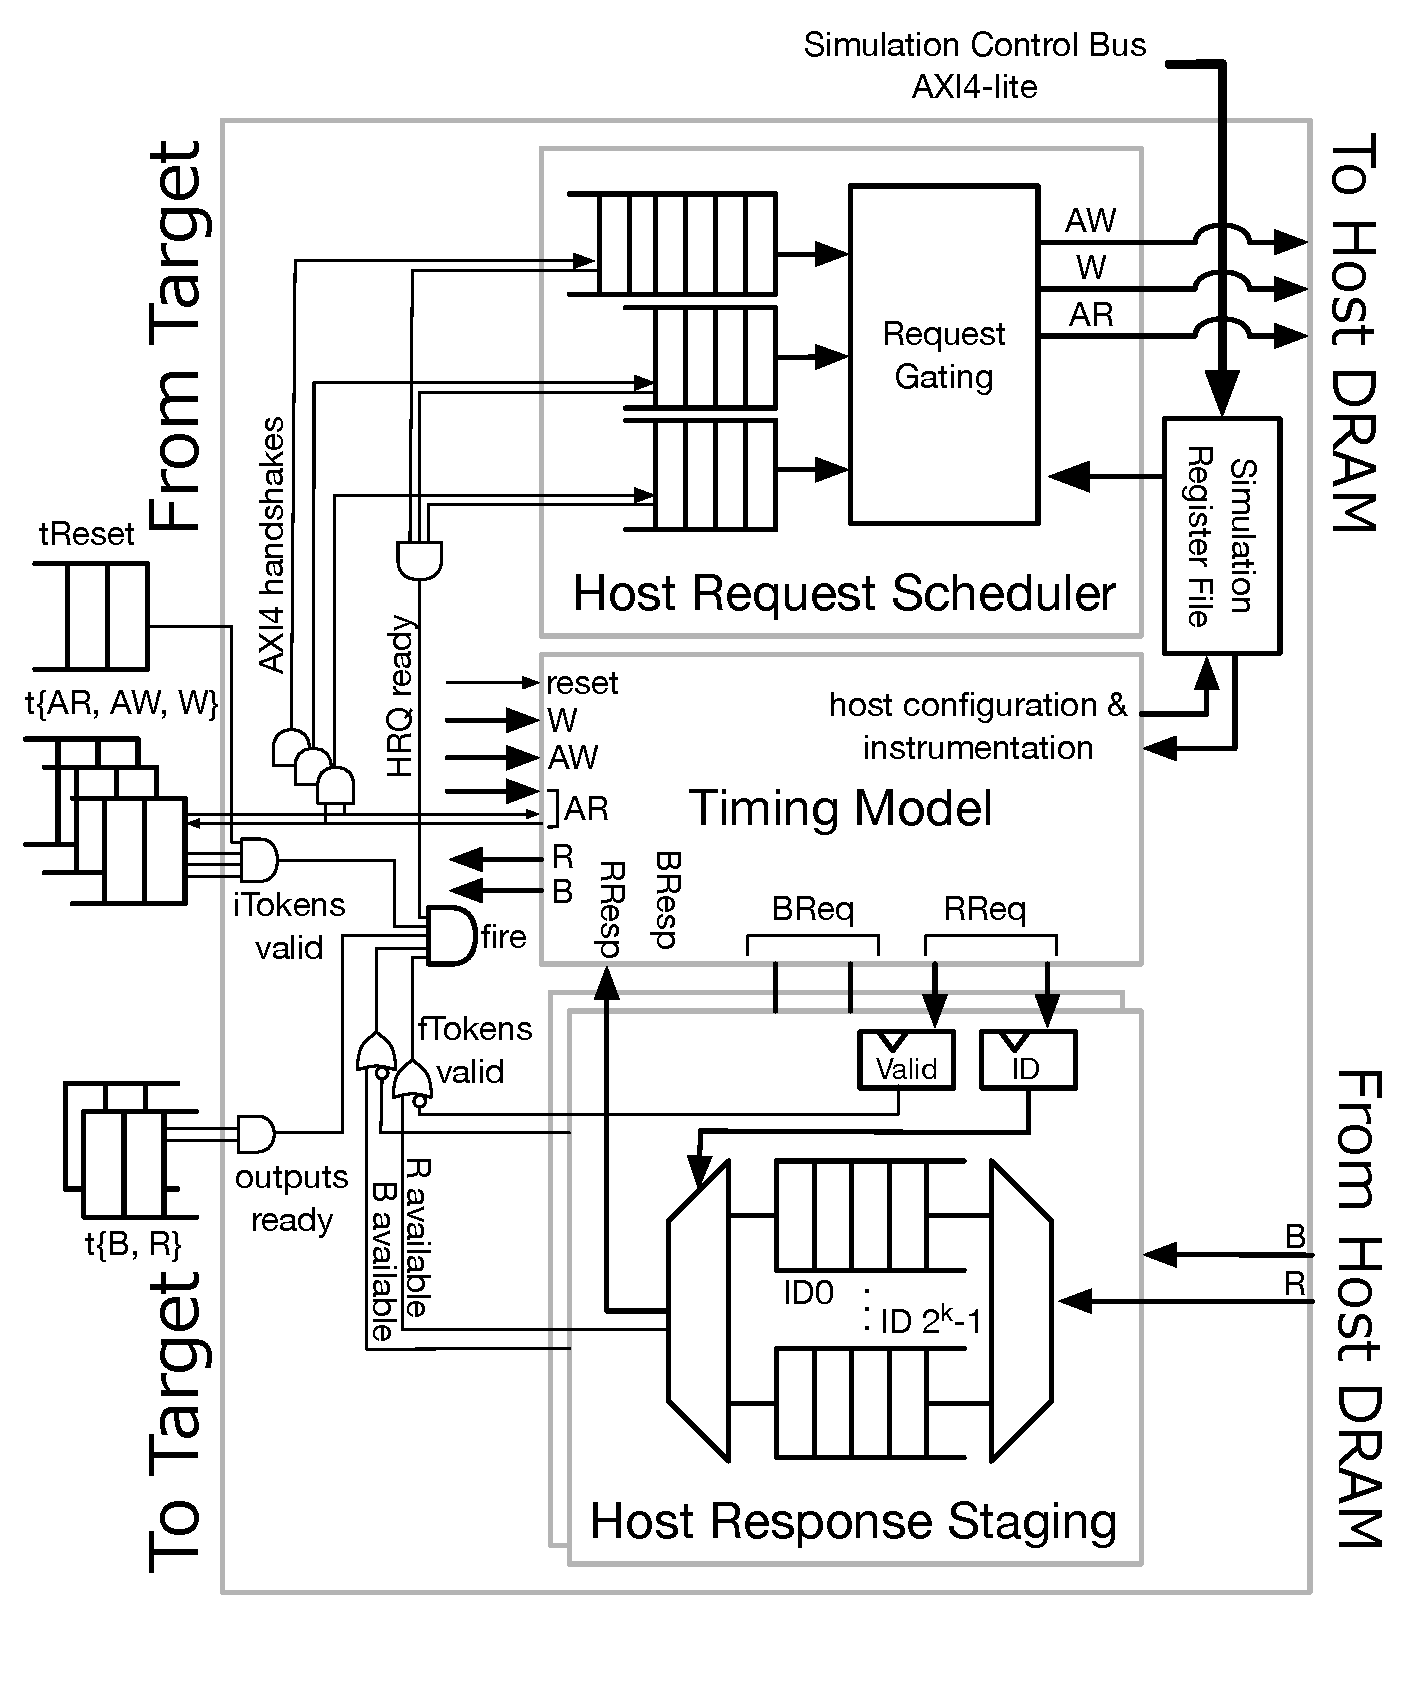
\includegraphics[width=\columnwidth]{figures/memory-model-block-diagram.pdf}
	\caption{Top-level diagram of memory system model with latency-bandwidth pipe timing model}
	\label{fig:timing_model}
\end{figure}

\section{Interfaces}

All instances of the model have three interfaces.

\begin{enumerate}
    \item \textbf{Target-Side} Host-decoupled AXI4 slave
        interface and synchronous reset. AXI4 consists of five ready-valid
        channels; three request channels driven by the master, and two
        reponse channels driven by the slave.  An input token consists of
        the valids and payloads for each request channel, the readies for
        each reponse channel, and the synchronous reset.  An output token
        is the complement; the valids and payloads for each response
        channel, and the readies for each request channel.  While tokens
        may be carried to and from the instance on seperate timing channels
        (for each AXI-4 channel and reset), simulation mapping ensures
        these are fused into a single input token, and fractured into
        multiple output tokens accordinly.

    \item \textbf{Host-Side} AXI4 master. This interface is used by the instance
        to make requests of the host memory system. It has no notion of target time.

    \item \textbf{Configuration-Side} AXI4-lite slave. This interface exposes both
        memory-mapped configuration registers and instrumentation to the
        simulation interconnect. During generation, the local memory map of the
        instance is produced and is included in the global simulation memory map
        in const.h.

\end{enumerate}

We selected AXI4 as it is the most common memory interface presented by FPGA IP
and widely implemented in ASICs. On the host-side, both major FPGA vendors
provide IP to bridge AXI4 to other standards, as well as adapters, to connect
master and slave devices that may have different interface widths. On the
target-side, the user will need to generate a bridge in their source RTL if
their design does not present and AXI4 master. In the future, we expect to
include target side interfaces for other interface specifications, like
TileLink.

The widths of all fields in target-side and host-side interfaces match, with
the exception of ARID and AWID. Here, the model can optionally reduce the
host-side ID width to the AXI4 specification's recommended maximum (4) or tie
it off altogether to prevent host-memory system reorderings. The model punts on
all other conversions, like target-to-host address translation, which will be
handled by the MIDAS compiler.

\section{Functional-Timing Split}

Like most previous FPGA-simulation work using custom RTL models, the generator
employs a timing-functional split. The egress and ingress units are functional:
they "emulate" target-memory system requests over a region of the host-memory
system of equal size. These units operate independently of target time and are
reused across all timing model classes. As the name suggests, the timing split
is captured entirely in the timing model.

The timing model interacts with the functional units in two places. Firsly,
through the simulation-side interface. Secondly, through the egress
request/response interface. Here, the timing model presents an AXI4 ID for the
host reponse it wishes to release to the target. The egress unit will reply
with the reponse if it is available, the timing model must fully dequeue the
reponse before requesting another\footnote{The AXI4 specification does not
permit interleaving of multiple read responses.}.

\begin{figure*}
	\centering
	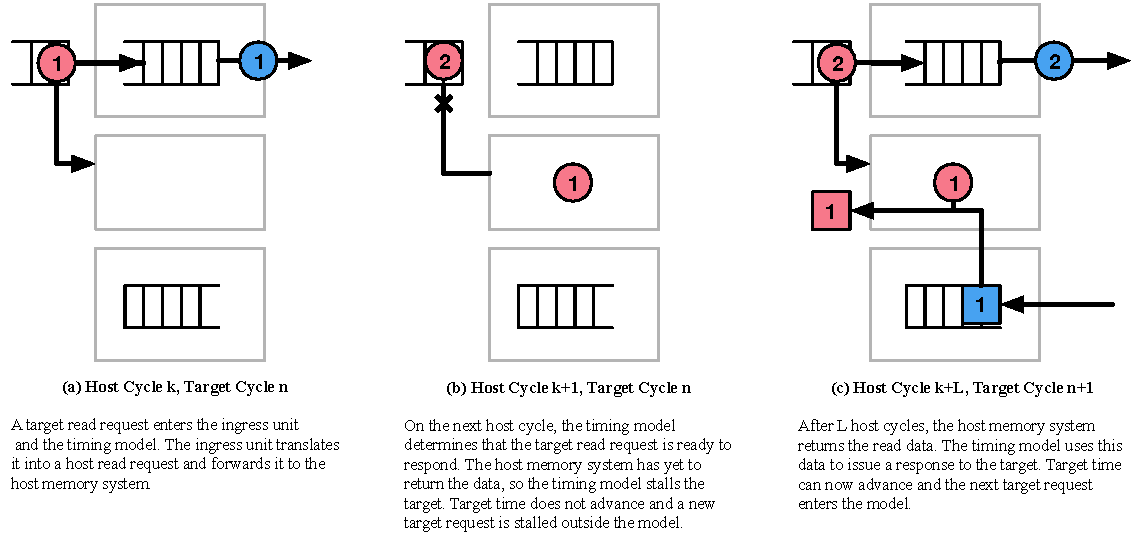
\includegraphics[width=0.8\textwidth]{figures/memory-model-operation.pdf}
	\caption{Operation of a single-cycle "magic" memory}
	\label{fig:model_operation}
\end{figure*}

\subsection{Egress Unit Design}\label{egress} Since both the host memory
system and the timing model may reorder responses\footnote{The AXI4
specification permits reordering of read and write responses across different
channels(different AXI4 IDs). Reponses within a particular channel must be
returned in the order they were requested. AXI4 imposes no ordering timing
constraints between read and write requests.} the egress unit implements a set
of virtual queues for each AXI4 channel. Each queue represents the FIFO
ordering within a single channel ID. The implementation of the virtual queues
differs based on:

\begin{itemize}
    \item Maximum number of outstanding requests
    \item Maximum number of AXI4 channels used by outstanding requests
    \item Minimum and maximum read request length
\end{itemize}

For a small number of IDs or a small number of outstanding requests, the
memory system model implements each virtual queue as a physical queue co-located in
the same BRAM. For greater numbers of AXI IDs, it dynamically assigns entries
within the BRAM to each response and maintains a list of pointers to those
entries for each channel ID.

\section{Configurability}

There are two points at which the model can be configured.  At
\textit{generation time}, the designer selects an instance. At
\textit{simulation time}, the instance is programmed through its
configuration-side interface to further set its behavior. Simulation time
configurability permits the designer to perform parameter sweeps without
needing to recompile the simulator bitstream -- at the expense of FPGA
resources. Since both timing and functional components of an instance are
provisioned pessimistically, giving hints to generator can greatly reduce FPGA
resource utilization. We outline some programmability-area tradeoffs here.

\begin{itemize}
    \item \textbf{Reducing functional component size.} The simulation designer
        can call out constraints on the behavior of the AXI masters to reduce
        the size of the ingress and egress units.  This achieved by putting
        bounds on the parameters defined in \ref{egress}.

    \item \textbf{Selecting the timing model class.} Simpler timing models
        consume fewer resources.

    \item \textbf{Reducing model programmability.} By default, each timing
        model class exposes all of its parameters as programmable registers on
        the simulation memory map. The generator permits tying particular knobs
        to static values, saving FPGA resources.

    \item \textbf{Reducing model instrumentation.} Model instances can be
        generated with instrumentation to track specific events and capture
        activity traces. This instrumentation is exposed on the simulation
        memory map. Generating the model with less instrumentation uses fewer
        resources.
\end{itemize}

\section{Timing Model Classes}\label{sec:timing_model}

The generator provides four base timing model classes:

\begin{itemize}
    \item \textbf{Latency-Bandwidth Pipe} Applies independently programmable
        latencies to read and write requests. The pipe does not accept any new
        requests beyond a programmable limit. This serves as a coarse-grain
        bandwidth bound via Little's law.

    \item \textbf{Bank Conflict} Adds a penalty of $max(0, t_{CP} -
        t_{\Delta})$ to a base latency if a read or write request used the bank
        $t_{\Delta}$ cycles prior, where $t_{CP}$ is the maximum conflict
        penalty.

    \item \textbf{FCFS DRAM MAS} Implements \ref{fcfs} with configurable open
        and closed page policy.

    \item \textbf{FR-FCFS DRAM MAS} Implements \ref{frfcfs} with an open page
        policy.
\end{itemize}

\TODO{Programmability charts}

Note that while the latter two models do have programmable $t_{RP}$, $t_{CS}$,
$t_{RCD}$, they are incomplete models of a generic DDR DRAM. For example, they
do not check against all DRAM timing constraints, nor do they model refresh.
They do, however, significantly improve modeling fidelity of DRAM memory
systems (with their respective MASs). We expect that the latency-bandwidth pipe
and bank conflict model will also suffice for modeling a slew of other memory
technologies to a first-order approximation.

